\chapter{Design And Implementation}

\section{Overall Design}
\par
#Our system is a blockchain based digital coupon validation system. The system
enables the retail chains to issue coupons. The retailers can verify the coupon
when the customer came to redeem it. It also makes the verification much more
efficient by enabling customers and retailers to verify the genuineness of the coupons. And there by enabling the solution to the customer loyalty issues.

\section{User Interfaces}
One of the main aims while designing the
system was to abstract as much lower level details of the system as possible
from the user. This system provides a web interface for its users. The interface is developed using NodeJS's Express framework.

\section{System Design}
\par
The only technology on earth today that could handle all these problems and provide us with immutable, verifiable and trustworthy certificates is ‘Blockchain’. The proposed system uses the public blockchain technology called Ethereum blockchain and the highly distributed. Here the focus is on solving the problem with the digital coupons storing and validation. This system provides the retailers to verify the genuinely of the coupons brought by the customer.
\subsection{Creating the discount coupon}
The authenticated retailer can add discount to a particular product with a particular time validity. Those data was hashed using the sha256 algorithm and was stored in an etherum blockchain.
The hashed code will be published and will be shared in various media in the form of a QR code for better representation. Whenever the retailer added a new discount coupon, he can create the respective coupons and will publish it. 

\subsection{Verifying the coupon}
The customer can bring those coupons and redeem them for a particular product. A coupon will only work for that particular product. All those constraint checking was done at the time of verifying. From the scanned QR code, the hash code will be detected, and it will be matched with the particular index of the deployed contract. By using the corresponding index, the aggregate data can be retrieved.
\begin{figure}[H]
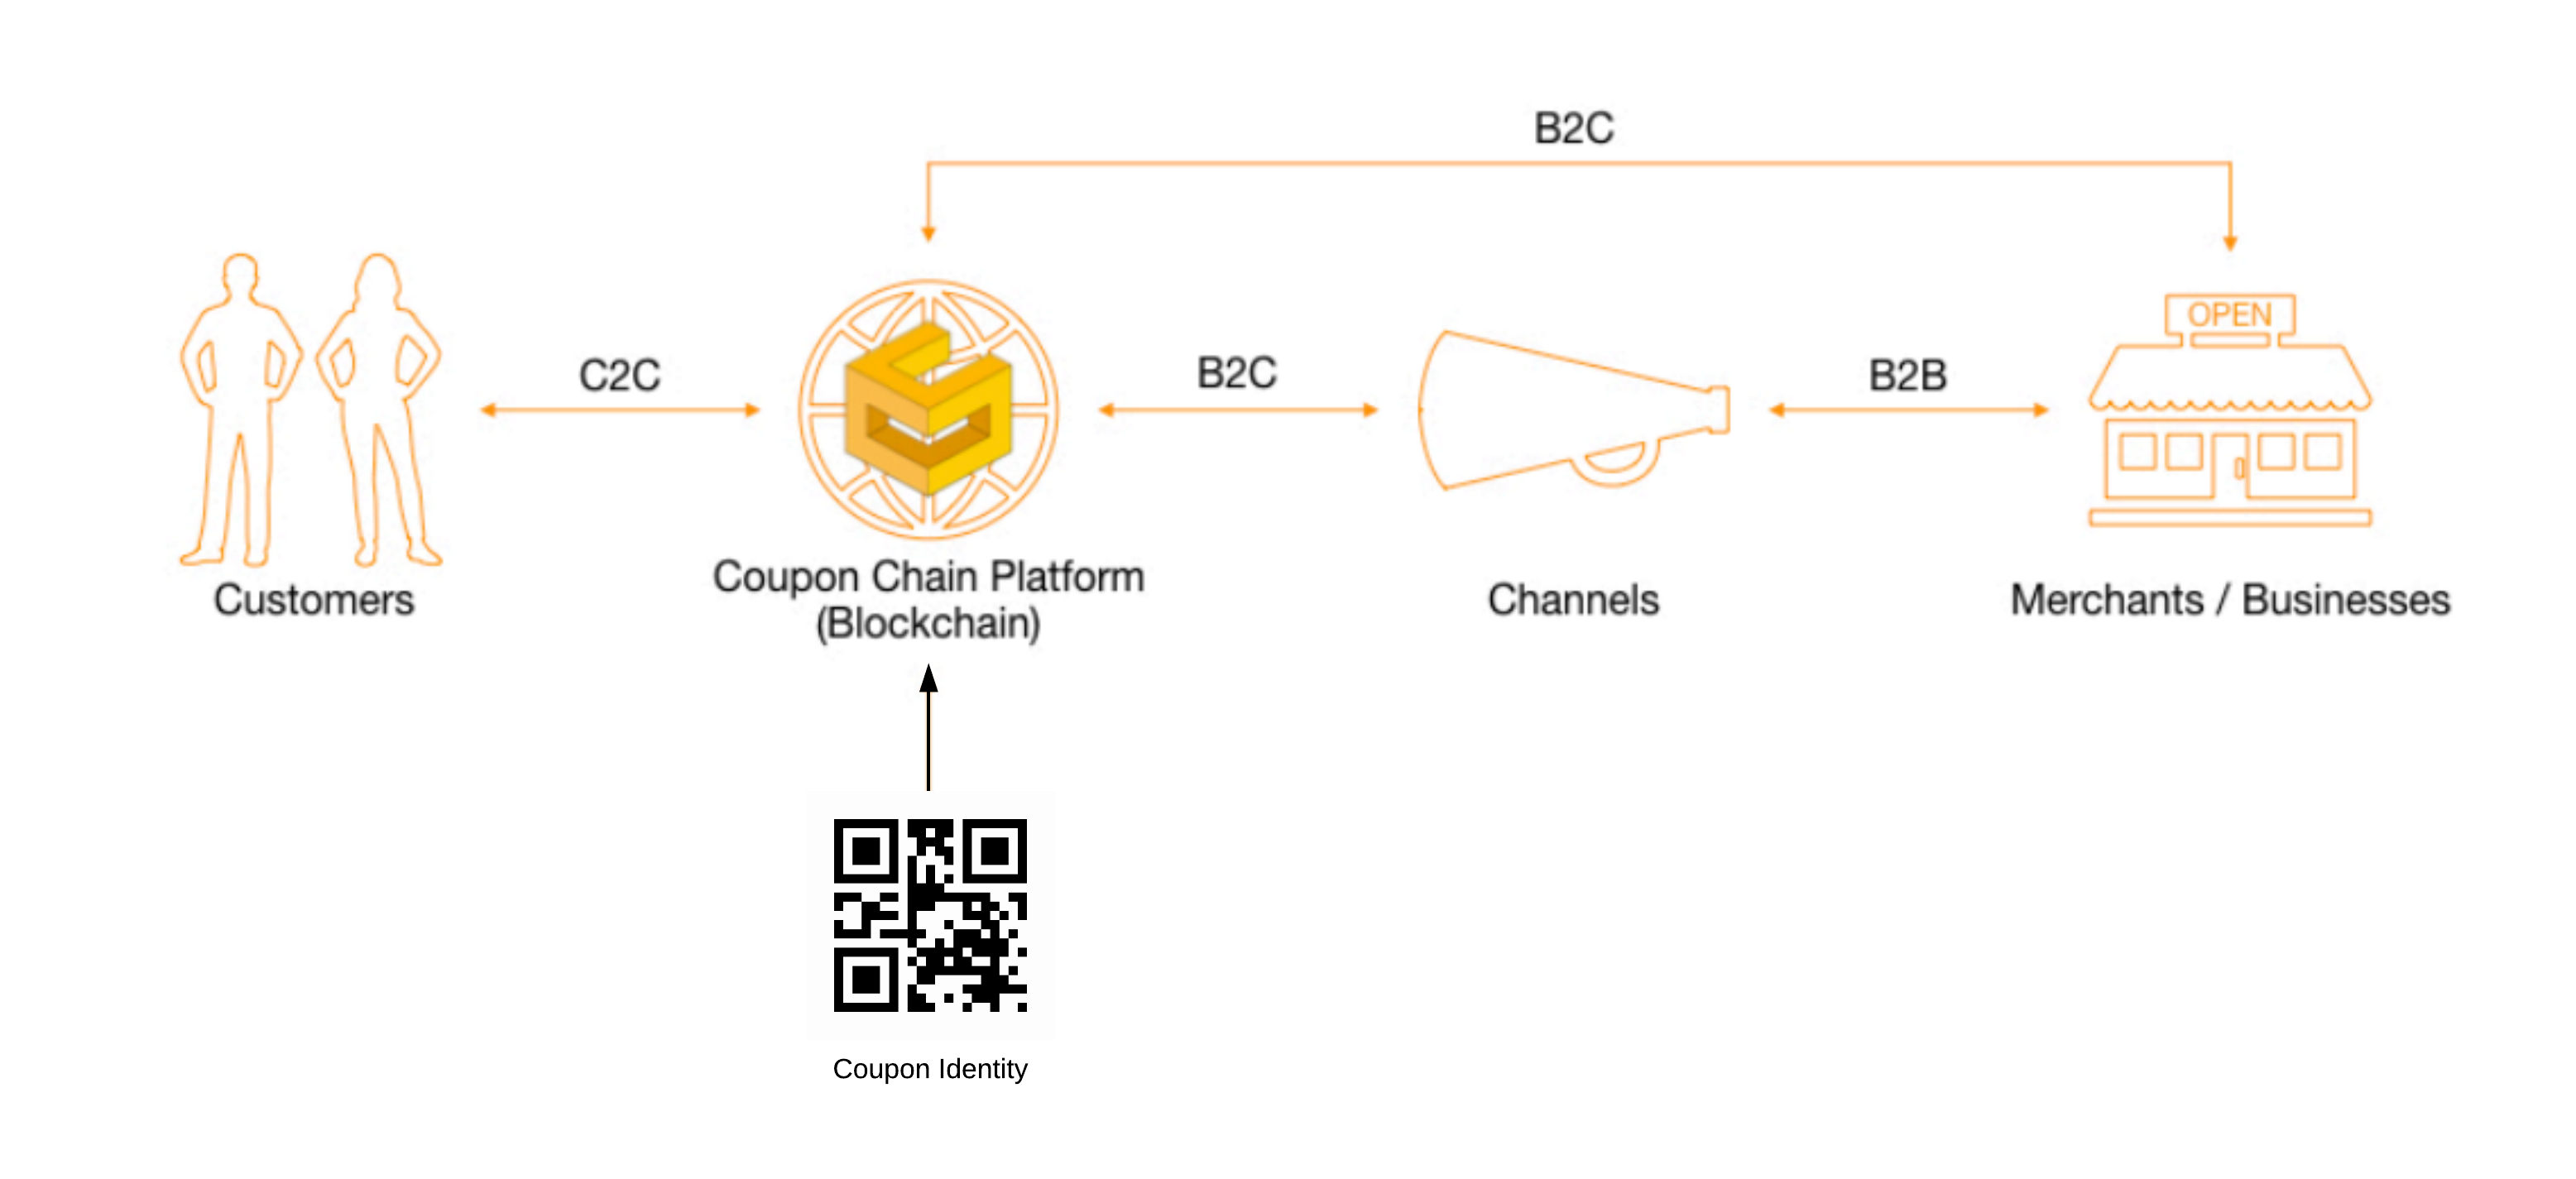
\includegraphics[scale=0.6]{flow}
\caption{Graphical flow}
\end{figure}

\section{Data Flow Diagrams for the System}
\par
These diagrams gives a clear picture about the privileges of each user. Also the entire working flow was specified in this. The DFDs are as follows:
\begin{figure}[H]
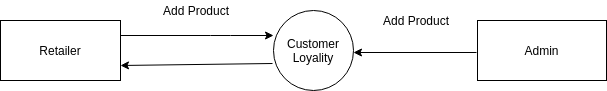
\includegraphics[scale=0.7]{level0_1}
\caption{Level 0.1 Data Flow}
\end{figure}

\begin{figure}[H]
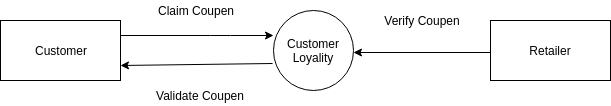
\includegraphics[scale=0.7]{level0_2}
\caption{Level 0.2 Data Flow}
\end{figure}


\hspace{2.0mm}
\begin{figure}[H]
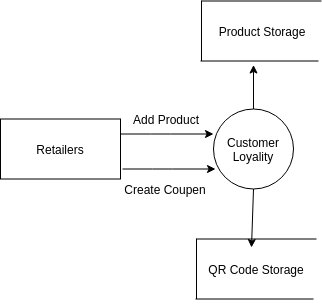
\includegraphics[scale=0.63]{level1_1}
\caption{Level 1.1 Data Flow}
\end{figure}
\vspace{2cm}
\begin{figure}[H]
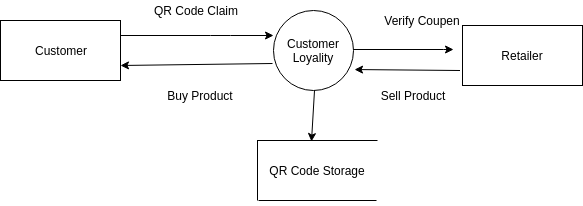
\includegraphics[scale=0.63]{level1_2}
\caption{Level 1.2 Data Flow}
\end{figure}
\newpage

\subsection{Screenshots}
screench0t 1 and 2
\newpage
scfreenshot 3 and 4
\newpage
scfreenshot 5 and 6




